\chapter{Mathematical introduction}
\label{chap:mathIntro}
The modern approach to the closed system dynamics is using \emph{differential geometry} formalism. Before we get to the quantum mechanics itself, let's introduce this formalism and recapitulate some definitions of this branch of mathematics. This chapter does not serve the full introduction to differential geometry, but reminds the essential realizations which should lead the reader to a better understanding of physical theory in the following chapters. Full introduction to differential geometry can be found for example in notes by \citet{krtous}, \citet{lu}, or \citet{fecko}. 
\section{Essentials}
Consider manifold $\M$ over the field of complex numbers $\mathbb C$. Curves on this manifold are parametrized by some real interval:
$$\mathcal J:\R \supset (P_i,P_f) \rightarrow \M,\; \qquad \xi\mapsto \mathcal J(\xi) \text{  for } \xi \in (P_i,P_f) .$$ 
The space of functions is $\FM\equiv\{f:\M\rightarrow \C\}$.


To define \bluee{\emph{vectors}} on $\M$, it is important to have some meaning of the \emph{direction}. The direction is defined using curves $\mathcal J_i$ satisfying 
$$\mathcal J_1(0)=\mathcal J_2(0)\equiv P$$
$$\der{}{t}x^i(\mathcal J_1(t))\big|_{t=0}=\der{}{t}x^i(\mathcal J_2(t))\big|_{t=0}.$$
Taking the equivalence class created by these two rules, sometimes noted as $\bluee{[\mathcal J]}$, we have an element of the tangent space to $\M$. We use standard notation for the \bluee{tangent space of $\M$} in some point $P\in\M$ as $\bluee{\T_P\M}$. Cotangent space is denoted as $\blueee{\T^*_P\M}$. Unifying all \bluee{tangent} and cotangent spaces over all $x$ we get tangent \bluee{$\TT\M$} and cotangent \blueee{$\TT^*\M$} bundle respective. To generalize this notation to higher tensors, we denote $\bluee{\TT\M}\equiv\TT^{\bluee{1}}\M$, $\blueee{\TT^*\M}\equiv \TT_{\blueee{1}}\M$. This gives us the possibility to increase the order, leading to $p-$times \bluee{contravariant} and $q-$times \blueee{covariant} tensors. These are denoted $\TT^{\bluee p}_{\blueee q} \M$. Tensor space in point $P\in\M$ is denoted ${\TT_P}^{\bluee p}_{\blueee q} \M$.
Using the congruence of curves on $\M$, the expression 
\begin{equation}
    \bluee{\der{}{\xi}}f\circ \mathcal J(\xi)\bluee{\Big|_{\xi=0}}
\end{equation}
has a good meaning, and we can define the \emph{vector} in some $P\in\M$ as
\begin{equation}
    \bluee{\bm v}: \FM\rightarrow \C \qquad f\mapsto \bluee{\bm v[}f\bluee ]\equiv \frac{\bluee \d f(\mathcal J(\xi))}{\bluee{\d \xi}}\bluee{\Big|_P} \equiv \bluee{\partial_\xi\Big|_P} f .
\end{equation}
It holds that $\bluee{\bm v}\in \bluee{\T_P\M}$ and can be expressed as the \emph{derivative in direction},
% \footnote{
%         The direction itself is usually denoted as
%         \begin{equation}
%             \frac{\D}{\d\bm\alpha}\mathcal J(\xi),
%         \end{equation}
%         where the "big D" notation is used to point out that it's not a classical derivative, but it maps curves to some entirely new space of directions.
%     } 
which can be understood in coordinates as
\begin{equation}
    \bluee{\bm v[}f\bluee ] = \bluee{\der{}{\bm v}} f\circ \mathcal J(\xi)\bluee{\Big|_{\xi=0}}=v^k\bluee{\der{}{x^k}} f(\bm x)\Big|_{P}.
\end{equation}
The directional derivative is denoted $\bm\nabla_v$
and in basis $\bluee{\bm e_i} \equiv \bluee{\partial/\partial x^i}$ it becomes
$$\bm\nabla=\bluee(\bluee{\bm e_1}, \bluee{\bm e_2},\bluee{\bm e_3}).$$


If needed, the \emph{abstract indices} (written by Greek letters) and \emph{pointer indices} (written using Latin letters) are differentiated. Abstract indices show the rank of the tensor, meaning \emph{how many empty slots for contraction the tensor has}. Pointer indices extract specific number from the tensor. For example
$$t^\mu_{\nu\kappa} \in \TT^1_2\M, \quad \text{ whilst for some }i,j,k\in\N: t^i_{jk}\in \mathbb C.$$
The summation over abstract and Latin indices has the same meaning. For \emph{Tensor contraction}, the index notation is used. When it is clear what type of tensors we are operating with, the Object notation can be used, for example $t(\bluee{\bm u},\bluee{\bm v})\equiv t_{\mu\nu}\bluee{\bm u^\mu \bm v^\nu}$. The contraction can also be noted using the contraction operator $\mathbf C$ when it is clear which indices are contracted or when it does not matter which of them are.

Now we have the notation to define one strong structure on manifolds — \emph{metric tensor}. 
\begin{definition}[Metric tensor]
If the 2-form $g_{\mu\nu}\in\TT^0_2\M$ is
\begin{itemize}
    \item linear in second argument: $\forall \alpha,\beta\in\C;\; \bluee{\bm u,\bm v,\bm w}\in \bluee{\TT^1\M}: \; g(\bluee{\bm u},\alpha\bluee{\bm v}+\beta \bluee{\bm w}) = \alpha g(\bluee{\bm u},\bluee{\bm v})+\beta g(\bluee{\bm u},\bluee{\bm w})$,
    \item hermitian: $\forall \bluee{\bm v,\bm w}\in \bluee{\TT^1\M}: \; g(\bluee{\bm v},\bluee{\bm w})=g(\bluee{\bm w},\bluee{\bm v})^*$,
    \item non-degenerate: $\forall \bluee{\bm v}\in\bluee{\TT^1\M}$ the function $\bluee{\bm w}\mapsto g(\bluee{\bm v},\bluee{\bm w})$ is not identically zero,
\end{itemize} 
we call $g_{\mu\nu}$ a \emph{metric tensor}. The \emph{star} $^*$ marks complex conjugation.
\end{definition}

We often require \emph{differentiable metric tensor}, or at least almost everywhere\footnote{Almost everywhere means \emph{with an exception to the submanifold of zero measure}.}. That assures that \emph{covariant derivatives} and \emph{parallel transport} are well-defined almost everywhere differentiable. 




Vectors of tangent space to some manifold can be compared only within one such space, and for that, they need to be transported to some common tangent space. The transport can be done using \emph{parallel transport} which is connected to the notion of \emph{covariant derivative}.

\begin{definition}[Covariant derivative]
\label{def:covariantDerivative}
    $\bm D_{\bluee{\bm v}}$ is called the covariant derivative in a direction $\bluee{\bm v} \in \bluee{\T_P\M}$, if $\forall f\in\FM, \; \bm A,\bm B\in \TT^{\bluee p}_{\blueee q} \M,\; \alpha\in\C: $
    \begin{itemize}
        \item $\bm D_{\bluee{\bm v}}:\; \TT^{\bluee p}_{P\blueee q} \M \rightarrow {\TT}^{\bluee p}_{\blueee q} \M$
        \item $\bm D_{f\bluee{\bm v}}\bm A=f\bm D_{\bluee{\bm v}} $ \emph(ultralocality in a direction\emph)
        \item $\bm D_{\bluee{\bm v}}(\bm A+\alpha \bm B)=\bm D_{\bluee{\bm v}}\bm A+\alpha\bm D_{\bluee{\bm v}}\bm B$ \emph(linearity in argument\emph)
        \item $\bm D_{\bluee{\bm v}}(\bm{AB})=(\bm D_{\bluee{\bm v}}\bm A)\bm B+\bm A(\bm D_{\bluee{\bm v}}\bm B)$ \emph(Leibniz rule\emph)
        \item $\bm D_{\bluee{\bm v}}(\mathbf C \bm A)=\mathbf C \bm D_{\bluee{\bm v}}(\bm A)$ \emph(commutation with contraction\emph)
        \item $\bm D_{\bluee{\bm v}}f=\bluee{\bm v[}f\bluee ]\equiv\bluee{\bm v^\beta \bm \d_\beta} f$ \emph(operation on functions\emph)
    \end{itemize}
\end{definition}

% \begin{definition}[Coavariant differential]
%     For $\bluee{\bm v} \in \bluee{\T_P\M}, \bm A\in \TT^{\bluee p}_{\blueee q} \M$, the covariant differential is defined as
%     $$\bm D:\; \TT^{\bluee p}_{\blueee q} \M \rightarrow {\TT_P}^{\bluee p}_{\blueee{q+1}} \M
%     \text{, for which } \bm D_{\bluee{\bm v}}\bm A^{\alpha\dots}_{\beta\dots}=\bluee{\bm v^\mathcal J} \bm D_{\mathcal J}\bm A^{\alpha\dots}_{\beta\dots}$$
% \end{definition}

% \begin{definition}[Pseudoderivative]
%     \label{def:pseudoderivative}
%         $\bm P$ is called a pseudoderivative of type $p,q$, if $\forall f\in\FM, \; \bm A,\bm B\in \TT^{\bluee p}_{\blueee q} \M: $
%         \begin{itemize}
%             \item $\bm P:\; \TT^{\bluee p}_{\blueee q}\M\rightarrow \TT^{\bluee p+m}_{\blueee q+n}\M$
%             \item $\bm P f=0$ (ultralocality)
%             \item $\bm P(f\bm A+\bm B)=f\bm P\bm A+\bm P \bm B$ (linearity)
%             \item $\bm P(\bm{AB})=(\bm{PA})\bm B+ \bm A(\bm{PB})$ (Leibniz rule)
%             \item $\bm M \mathcal C \bm A=\mathcal C\bm{MA}$ (commutation with contraction)
%         \end{itemize}
% \end{definition}
    
\begin{definition}[Parallel transport]
    Parallel transport of tensors in tensor field $\bm A\in \TT^{\bluee p}_{\blueee q} \M$ along some path $\mathcal J$ going from $P_i\in\M$ to $P_f\in\M$ is denoted
    \begin{align*}
        \Par_{\mathcal J}:\; {\TT _{P_i}}^{\bluee p}_{\blueee q}\M&\rightarrow {\TT_{P_f}}^{\bluee p}_{\blueee q}\M\\
        \bm A|_{P_i} &\mapsto (\Par_{\mathcal J} \bm A)|_{P_f}.
    \end{align*}
\end{definition}
This means that the parallel transport takes a tensor at some ${\TT_{P_i}}^{\bluee p}_{\blueee q} \M$ and transports it to ${\TT_{P_f}}^{\bluee p}_{\blueee q} \M$.  Those two tensors belong to the same tensor field, but are essentially different. One cannot simply add or subtract them. For that they need to be parallel transported into the same tensor space $\TT^{\bluee p}_{\blueee q} \M$.

% \begin{definition}[Coordinate derivative]
%     Associate the derivative $\bm \partial$ with coordinates $x^\mu$ on some $O\subset\M$ as
%     $$\bm \partial (\bm \d x^j)=0.$$
% \end{definition}
% Then the coordinate derivative of any tensor can be expressed as
% \begin{equation}
%     \bm \partial_\rho \bm A^{\alpha,\dots}_{\beta\dots} = \bm A^{a,\dots}_{b\dots,q}\bm \d_\alpha x^q \bm \d_\alpha x^b  \dots \frac{\bm \partial^\beta}{\bm \partial x^a},
% \end{equation}
% where on the expression on the left means \emph{taking the covariant derivative of the tensor} and the expression on the right \emph{multiplying the basis of the tensor space by derivative of the elements of tensor $\bm A$}.
% \begin{thm}[Difference of covariant derivatives]
%      Difference of two covariant derivatives, i.e. two objects $\bm  D$, $\bm{\tilde D}$ satisfying Def. \ref{def:covariantDerivative},
%       $$\bm D-\bm{\tilde D}$$
%     is a pseudoderivative from Def. \ref{def:pseudoderivative}.
% \end{thm}

Another object needed for calculating the covariant derivative is \emph{affine connection}. It is generally defined as the difference between covariant and coordinate derivative
$\bm \Gamma\coloneqq \bm D-\bm\partial$. Because this definition requires some additional theory, only the \emph{connection on metric spaces} is provided here.

\begin{definition}[Connection and Christoffel symbols]
The Affine connection on metric spaces can be defined as
    \begin{equation}
        \Gamma^{\alpha}_{\;\mu\nu} \coloneqq \frac{1}{2}g^{\alpha \beta}\left(g_{\beta\mu,\nu}+g_{\nu\beta,\mu}-g_{\mu\nu,\beta}\right),
    \end{equation}
    where \emph{comma notation} for coordinate derivative is used. Its elements are called the \emph{Christoffel symbols}.
\end{definition}
    The covariant derivative of a vector $\bluee{\bm a}\in \T_P\M$ for manifold with coordinates $x^\mu$ can be expressed as
    \begin{equation}
        \Der{\bluee{\bm a^\mu}}{x^\nu}=\bluee{\bm a_{\;,\nu}^\mu}-\Gamma^\mu_{\alpha\beta} x^\alpha \bluee{\bm a^\beta}
    \end{equation}
    and for $\blueee{\bm\alpha\in} \T_P^*\M$ it is
\begin{equation}
    \Der{\blueee{\bm \alpha_\mu}}{x^\nu}=\blueee{\bm \alpha_{\mu,\nu}}-\Gamma^\alpha_{\mu\beta}x^\beta \blueee{\bm \alpha_\alpha}.
\end{equation}

The vector $\bluee{\bm v}\in \T_P\M$ is said to be parallel transported along curve $\mathcal J(\lambda)$, if its covariant derivative vanishes along $\mathcal J(\xi)$, meaning
\begin{equation}
    \Der{\bluee{\bm v^\mu}}{\xi}=0.
\end{equation}

\section{Fiber bundle}
\label{sec:bundleDef}
Sometimes one needs to add additional structure to every point on the manifold. At every point of the manifold we introduced a tensor space. This structure can be described by so-called \emph{fiber bundles}.
\begin{definition}[Fiber bundle]
    \label{def:fiberBundle}
    Structure 
\begin{center}
    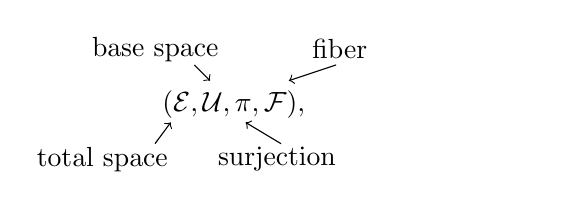
\begin{tikzpicture}[remember picture]
        \node {\(\displaystyle(
            \mathcal{E},\mathcal{U},\pi,\mathcal{F}),
            \)};
            \node[text width=3cm] at (-1,-0.7) {total space};
            \node[text width=3cm] at (1.3,-0.7) {surjection};
            \node[text width=3cm] at (-0.3,0.7) {base space};
            \node[text width=3cm] at (2.5,0.7) {fiber};
            \draw[->] (-1,-0.5)--(-0.8,-0.23);
            \draw[->] (-0.5,0.5)--(-0.3,0.30);
            \draw[->] (0.6,-0.5)--(0.15,-0.23);
            \draw[->] (1.3,0.5)--(0.7,0.3);
        \end{tikzpicture}
\end{center}
    for topological spaces $\mathcal{E}$, $\mathcal{U}$, $\mathcal F$ and continuous surjection $\pi: \mathcal{E}\rightarrow \mathcal{U}$ satisfying a local triviality, is called a \emph{Fiber bundle}. The local triviality means that $\mathcal{U}$ is connected\footnote{Connected mean, it can't be represented as a union of two and more disjoint sets} and for every $x\in \mathcal{U}$, there is an open neighborhood $\mathcal{N}\subset \mathcal{U}$ \emph{(trivializing neighborhood)} such that there exists a homeomorphism from $\mathcal{N}$ to so-called \emph{product space}
    $$\phi: \pi^{-1}(\mathcal{N})\rightarrow \mathcal{N}\times \mathcal{F},$$
    such that $\pi^{-1}\circ \pi(\mathcal{N})=\mathcal{N}$. Plus there exist natural projection from $\mathcal{N}\times \mathcal{F}$ to $\mathcal N$, setting the coordinate in fibers to zero. The structure can be visualized as follows: 
    % See the mappings in Fig. \ref{fig:bundle}.

    \begin{figure}[H]
        \centering
        \begin{tikzpicture}[->,>=stealth',auto,node distance=3.0 cm,
            thick,main node/.style={}]
            
            \node[main node] (1) {$\pi^{-1}(\mathcal U)$};
            \node[main node] (2) [right of=1] {$\mathcal U$};
            \node[main node] (3) [right of=2] {$\mathcal U\times \mathcal F$};
            
            \path[every node/.style={}]
            (1) edge node [above] {$\pi$} (2)
            (3) edge node [above] {projection} (2)
            (1) edge[bend right] node [below] {$\phi$} (3);
        \end{tikzpicture}
    \end{figure}

\end{definition}
Because the projections of products are open maps, $\pi: \mathcal{E}\rightarrow \mathcal{N}$ must be an open map. The manifolds at every point $x\in \mathcal{F}$ are all locally diffeomorphic to each other.

These structures are usually imagined like fibers from the manifold, similar to your head's hair. One can imagine the $\mathcal N$ as head, $\mathcal F$ the hair, $\pi$ applied on any point on hair returns the point on the head, and $\mathcal E$ is the head with all the hairs. This analogy holds only if all hairs are the same.


% \section{\red{Vector Bundle}}
% Conversely, given a fiber bundle (E, X, $\pi$, Rk) with a GL(k) cocycle acting in the standard way on the fiber Rk, there is associated a vector bundle. This is sometimes taken as the definition of a vector bundle


% \subsection{Connection on vector bundles}
% \citep{lu}[chap. 10.1]
% Connection maps vector from tangent space to base manifold $\mathcal{X}$ with some element from total space $\mathcal{E}$ to total space
% $$\Gamma: \mathcal{X}\times \mathcal{E}\rightarrow \mathcal{E}$$
% such, that
% \begin{itemize}
%     \item $\Gamma_X s$ is $\mathcal{F}-$linear in $X$ and $\R-$linear in $s$
%     \item Leibniz rule for $f\in \mathcal{C}^\infty$ is satisfied: $\Gamma_X(f s) = (X f)s+f\Gamma_X s$
% \end{itemize}


% \subsection{Metric on vector bundles}
% Map
% $$g_{\mu\nu}: \mathcal{N}\times \mathcal{N} \rightarrow \R$$

% \section{\red{Sections}}
% \label{sec:section}
% \emph{Section} is a function
% $$f:\mathcal{N}\rightarrow \mathcal{F},$$
% such that $\pi(f(x))=x$ for $\forall x\in \mathcal{N}$. This defines new manifold cutting throw $\mathcal{E}$.

% \textcolor{red}{Sectioning of fiber bundles creates vector spaces}


% \section{Pull-back and push forward}
% Push-forward and pull-back are used to transport vectors and covectors between manifolds. Let's have two manifolds $\M$, $\mathcal{N}$, a smooth mapping $\phi$ and functions $f,\tilde f$ such that
% \begin{align*}
%     \phi&:\M\rightarrow \mathcal{N}\qquad x\mapsto \phi x\\
%     \tilde f&:\mathcal{N}\rightarrow \R 
% \end{align*}
% \emph{Pull-back of the function} then defines a new function $
% f:\M\rightarrow \R $ as
% $$\phi^*:\F \mathcal{N}\rightarrow \F\M \qquad  \tilde f\mapsto f=(\phi^*\tilde f)(x)\equiv \phi^*\tilde f(x) =\tilde f(\phi x).$$
% \emph{Push-forward of a vector} is defined as
% $$\phi_*: \T_x\M \rightarrow \T_{\phi x}\mathcal N\qquad \phi_* 
% \Der{\mathcal J(\xi)}{\xi}\Big|_x=\Der{\phi \mathcal J(\xi)}{\xi}\Big|_x$$
% and \emph{pull-back of a covector} $\bm\tilde\alpha\in \T_{\phi x}\mathcal N$ is
% $$\phi^*: \T_{\phi x}\mathcal N\rightarrow \T_x\M  \qquad (\phi^*\bm \tilde\alpha)_\mu v^\mu\big|_x= \tilde\alpha_\mu (\phi_* \bm v)^\mu\big|_{\phi x}.$$
% If $\phi$ has a smooth inversion, i.e. it is a dippheomorphism, we can define pull-back of vectors as
% \begin{equation}
%     \phi^*=\phi_*^{-1}
% \end{equation}
% and push-forward of covectors
% \begin{equation}
%     \phi_*=(\phi^{-1})^*
% \end{equation}




% \section{\red{Parallel transport on vector bundles}}
% \textcolor{blue}{this is what we need}
% Parallel transport of vector $V$ along curve $\mathcal J$ will be denoted
% $$\Par_{\mathcal J} V.$$



% \section{\red{Antisymmetric tensors}}
% $p-$form $\bm A\in \TT_p \M$ is called \emph{antisymmetric}, if changing the order of the indices has impact only on the sign, symbolically
% $$A_{i_1\dots i_p} = \sign(\sigma)A_{i_{\sigma_1}\dots i_{\sigma_p}},$$
% where $\sigma$ is some permutation.\emph{Antisymmetrisation} is defined as a normalized sum over all permutation
% \begin{equation}
%     A^{[i_1\dots i_p]}\equiv \frac{1}{p!}\sum_\sigma A^{[i_{\sigma_1}\dots i_{\sigma_p}]}. 
% \end{equation}

% The \emph{wedge product} of $A\in \TT_p \M$ and $B\in \TT_q \M$ is antisymmetrisation of the tensor product in the sense
% \begin{equation}
%     A\wedge B\equiv \frac{(p+q)!}{p!q!} A^{[i_1\dots i_p}\otimes B^{i_1\dots i_q]}
% \end{equation}

\section{Riemannian geometry}
Some Riemannian geometry theorems have implications in the theory of quantum driving. First, some basic definitions are needed.

\begin{definition}[Riemannian manifold]
    Manifold is called Riemannian if it is equipped with a positive definite metric tensor.
\end{definition}
\begin{definition}[Connected manifold]
    A manifold is connected if the distance between two points is the infimum of the lengths of curves joining the two points.
\end{definition}
\begin{definition}[Compact manifold]
    A manifold is said to be compact if its every open cover has a finite subcover.
\end{definition}
\begin{definition}[Geodesical completeness]
    A manifold is said to be geodesically complete if every geodesic on it can be extended to infinite values of their affine parameter. 
\end{definition}
The geodesical completeness is a coordinate-independent notion.
\begin{definition}[Geodesic maximality]
    A manifold is said to be geodesically maximal if it is either geodesically complete or every non-complete geodesic (such that cannot be extended to infinite values of their affine parameter) ends in a singularity.
\end{definition}
Geodesic maximality is a coordinate-dependent notion only if the manifold is geodesically complete.


\begin{thm}[Von Neumann-Wigner]\emph{\citet[page 305]{landau}}
    \label{thm:n-2}

    This, sometimes called the Non-Crossing Theorem, states that the eigenvalues of the Hermitian matrix driven by $N$ continuous real parameters forms at a maximum $(N-2)$-dimensional submanifold.
\end{thm}


\begin{thm}[Hopf-Rinow Theorem]\emph{\citet[page 125]{petersen}}
    \label{thm:hopf-Rinow}


    For connected Riemannian manifold $\M$ with the metric $g$, following are equivalent:
    \begin{itemize}
        \item $(\M,g)$ is geodesically complete, i.e., all geodesics are infinite,
        \item $(\M,g)$ is geodesically complete at some point $P$, meaning the geodesics going through $P$ are infinite,
        \item $(\M,g)$ satisfies the Heine-Borel property, i.e., every closed bounded set is compact,
        \item $(\M,g)$ is complete as a metric space.
    \end{itemize}
\end{thm}
\begin{thm}[Modified Hopf-Rinow Theorem]\emph{\citet[Chapter 3]{claudio}}
    \label{thm:hopf-Rinow_modified}

    For connected Riemannian manifold $\M$ with the metric $g$, any two points on $\M$ can be joined with a minimizing geodesic.
\end{thm}
This generally means that in a space with singularity exists such points, which cannot be connected with the rest of the manifold using geodesics. In General relativity, this area is, for example, below the event horizon of black holes.

\begin{thm}[On completeness]\emph{\citet[Chapter 3]{claudio}}
    \label{thm:compact}
    
    A compact Riemannian manifold is geodesically complete.
\end{thm}





An important tensor in differential geometry is the \emph{Riemann tensor}
\begin{equation}
    R^\alpha_{\;\;\beta\gamma\delta}\coloneqq \Gamma^\alpha_{\;\;\beta\delta,\gamma}-\Gamma^\alpha_{\;\;\beta\gamma,\delta}+\Gamma^\mu_{\;\;\beta\delta}\Gamma^\alpha_{\;\;\mu\gamma}-\Gamma^\mu_{\;\;\beta\gamma}\Gamma^\alpha_{\;\;\mu\delta}.
\end{equation}
\emph{Ricci tensor} can be defined as its contraction 
\begin{equation}
    R_{\alpha\gamma}\coloneqq R^\mu_{\;\;\alpha\mu\gamma},
\end{equation}
which is second order symmetric tensor.
\emph{Ricci scalar}, describing the curvature on manifold, is defined as contraction of the Ricci tensor
\begin{equation}
    R\coloneqq R^\mu_{\;\;\mu}.
\end{equation}


\section{Geometry in 2 dimensions}
Ricci scalar can be simplified for 2-dimensional manifold as
\begin{equation}
    R=\frac{2}{g_{22}}\left(\Gamma^1_{\;22,1}-\Gamma^1_{\;12,2}+\Gamma^1_{\;11}\Gamma^1_{\;22}+\Gamma^1_{\;12}\Gamma^2_{\;22}-\Gamma^1_{\;21}\Gamma^1_{\;12}-\Gamma^1_{\;22}\Gamma^2_{\;12}\right).
    \label{eq:Ricci2D}
\end{equation}
Another possibility to express the Ricci tensor in two dimensions, see \citet[eq. 6,7]{geometricTensorLipkin}, is
\begin{equation}
    R=\frac{1}{\sqrt{\abs{g}}}(\mathcal{S}+\mathcal{T}),
\end{equation}
for
\begin{align}
    \mathcal{S}&\coloneqq \left(\frac{g_{12}}{g_{11}\sqrt{\abs{g}}}g_{11,2}-\frac{1}{\sqrt{\abs{g}}}g_{22,1}\right)_{,1}\\
    \mathcal{T}&\coloneqq \left(\frac{2}{\sqrt{\abs{g}}}g_{12,1}-\frac{1}{\sqrt{\abs{g}}}g_{11,2}-\frac{g_{12}}{g_{11}\sqrt{\abs{g}}}g_{11,1}\right)_{,2}.
\end{align}
% This equation turned out to be less numerically stable, therefore Eq. \ref{eq:Ricci2D} is used later on for calculating the Ricci tensor.

